\subsection{Product Perspective}
The aim of SafeStreets is to increase the security around the streets of the cities also simplifying the interventions of the authorities. \newline
In order to make this possible, the application must include some functionalities that helps determining for a report is real or fake. \newline
To monitor the position of the user sending the violation report, SafeStreets will exploit device’s available GPS sensor and will also include a detailed map where users can discover the most unsafe areas or streets. \newline
To allow users to take pictures of the violation, the application will use the camera nowadays inserted in every smartphone. \newline
SafeStreets will also need a stable connection to the internet in order to send violation reports or to mine data from the database. \newline\par
In order to differentiate functionalities for the various types of users, the application will be accessible by two different clients (basic users and authorities). \newline
Basic users needs to insert personal informations (eg. SSN) during the sign-in process to reduce the number of false reports. \newline
Authorities, on the other hand, must insert authentication data (eg. Police service number) during the sign-in process to ensure that the data won’t be accessed by not authorised people. \newline
Depending on the kind authority, SafeStreets offers different levels of data visibility.

\subsubsection{Class Diagram}
The high-level class diagram provides a model of the application domain, containing the most important classes that will be necessary to build the system. 
\begin{figure}
	\centering
	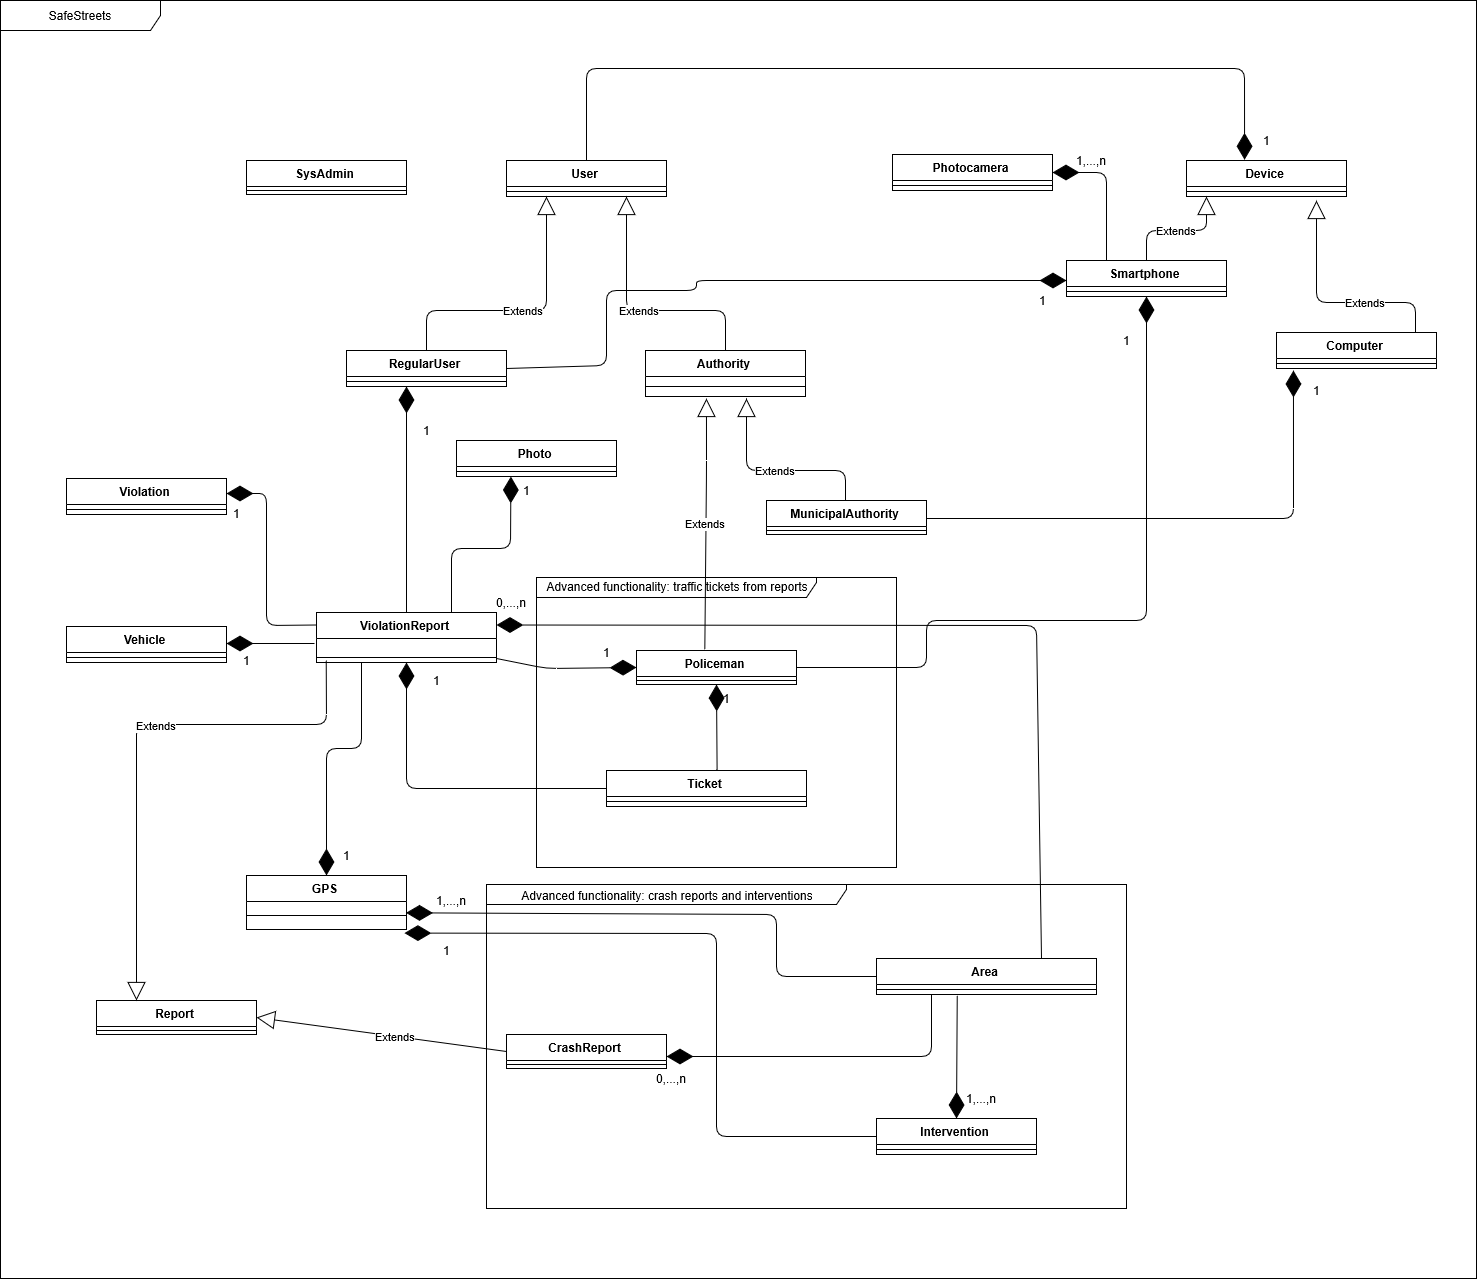
\includegraphics[width=\textwidth]{Images/ClassDiagram.png}
	\caption{\label{fig:metamodel2}Class diagram}
\end{figure}

\subsubsection{Statecharts}
Now we will analyse the most critical aspects of the application workflow, modelling their behaviours using state diagrams.
\\ \\
Me: *inserts the image of the state diagrams* 

\subsection{Product Functions}
In this section we analyse the main functions of SafeStreets: 
\begin{itemize}
	\item Data Management: \\ \\
	The users must give the application the permission to access their data and device’s functionalities, such as GPS position and Camera. \\
	They are also asked to insert personal data (eg. SSN) during the account registration phase. \\
	If these requirements are met, SafeStreets allows authenticated users to send violation reports including geographical position and pictures of the violation. \\
	All this data is then used to check the veracity of a report and to help the authorities to identify the violator. \\
	On the other hand the authorities must insert authentication data in order to access the information stored by SafeStreets. \\
	The system must be also able to use stored data about tickets issued by the local police to build statistics.
	
	\item Report management: \\ \\
	One of the main features of SafeStreets is the possibility for users to send reports about the traffic violations that occurs around them. \\
	The system must be able to automatically decide wether a report must be discarded or kept in memory. \\
	The reasons for reports to be discarded are basically two: the report is fake (or not appropriate) or the same violation has already been reported (same photo for two different violations). 
	
	\item user management: \\ \\
	The system includes two different clients for the login of the different type of users. \\
	One is used by basic users that can send reports and discover the unsafe areas of the city, the other is used by registered authorities to mine data about reports or possible interventions to reduce violations. 
	
	\item possible intervention suggestions \\ \\
	SafeStreets must be able to automatically suggest possible interventions to avoid traffic violations in the most unsafe areas. \\
	The suggestions will be more accurate the more reports are sent from the same area. \\
	For example, if the applications receives a lot of reports about cars parked on the bike lane, there might be need of a barrier between the street and the lane. 
	
	\item information crossing \\ \\
	The system must be able to cross its data with informations about car accidents coming from the municipality. \\
	This functionality can be useful to identify the most dangerous areas or to accurately suggest interventions.  
\end{itemize}

\subsection{User Characteristics}
Here is a list of the actors of the application: 
\begin{itemize}
	\item Basic users: Every authenticated user that is able to send violation reports and mine the application data to know the most unsafe areas. 
	\item Local police users: Users with a police service number able to access data about reports sent by the basic users. 
	\item municipalities: authorised users from the municipality of a city able to mine more detailed data such as the possible interventions suggested by SafeStreets. 
\end{itemize}

\subsection{Assumptions, dependencies and constraints }
\begin{itemize}
	\item (D1) Users’ devices are connected to the internet 
	\item (D2) Users’ devices are equipped with a working camera 
	\item (D3) GPS signal is always available on users’ devices 
	\item (D4) Every user can provide a unique id 
	\item (D5) Only verified reports are accepted 
	\item (D6) Users that want to access authorities’ data must be acknowledged institutions 
	\item (D7) Car’s license plates are unique 
	\item (D8) Every license plate is related to one and only one person
\end{itemize}
 